\subsection{Beamspot Calibration}

\subsubsection{Beamspot Overview}

The \emph{beamspot} in CMS is the luminous region where the two beams interact.
This region is described by a probability density function $\rho(x,y,z)$ for the pp collisions;
to first approximation, the $\rho$ is given by a three-dimensional gaussian function that can be visualised as a tri-axial ellipsoid \cite{CMS-PAS-TRK-10-005}.
In ideal conditions, the beamspot would be centered in,
and its axes would be aligned to,
to the detector's reference frame.
During real operation, the beamspot is displaced and rotated along all axes,
which are represented by a displacement vector and a set of Euler angles.
Those quantities can be translated to the following observables, the \emph{beamspot parameters}:
\begin{itemize}
\item the centroid position $x_{\text{BS}}, y_{\text{BS}}, z_{\text{BS}}$,
\item the transverse widths $\sigma_{x}, \sigma_{y}$,
\item the longitudinal width $\sigma_{z}$,
\item and the tilts with respect to the $z$ axes: $\frac{dx}{dz}$, $\frac{dy}{dz}$.
\end{itemize}
Figure~\ref{fig:beamspotCartoon} shows the a diagram of the ideal and real beamspot.
\begin{figure}[htbp]
   \centering
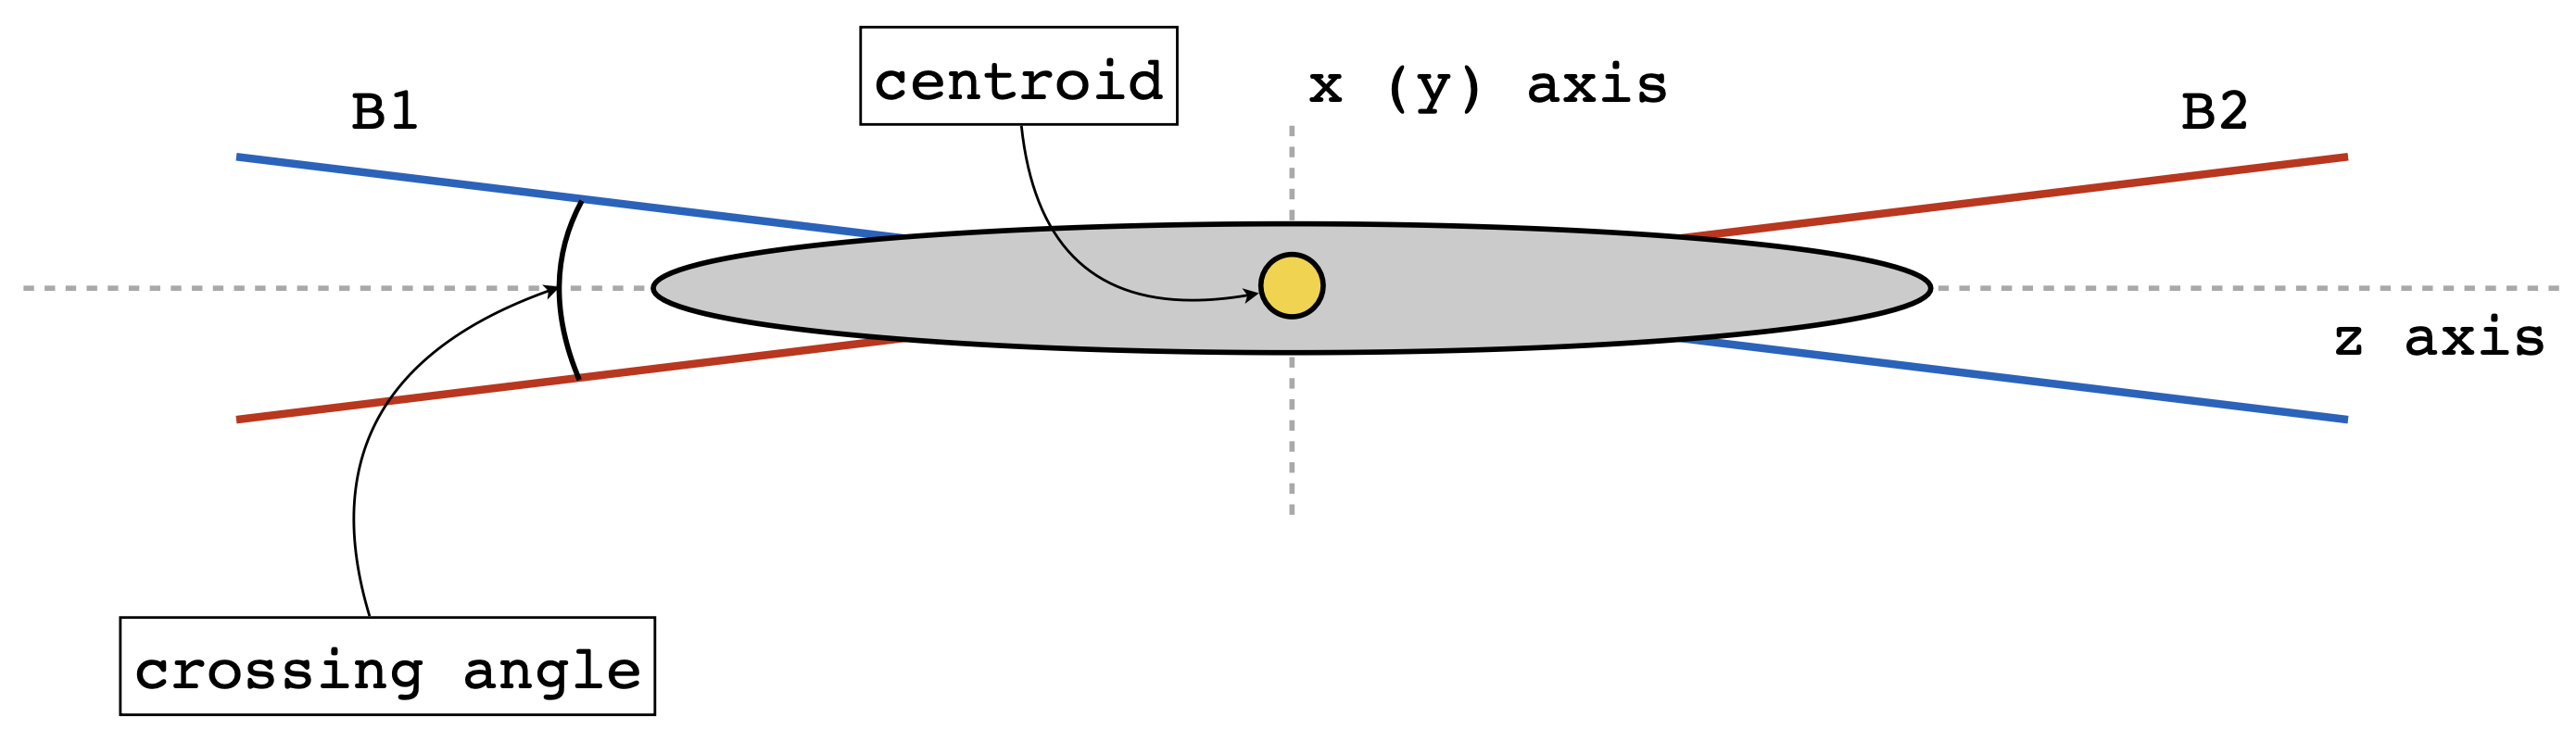
\includegraphics[width=0.7\textwidth]{figures/IdealBeamspot.png}\\[3ex]
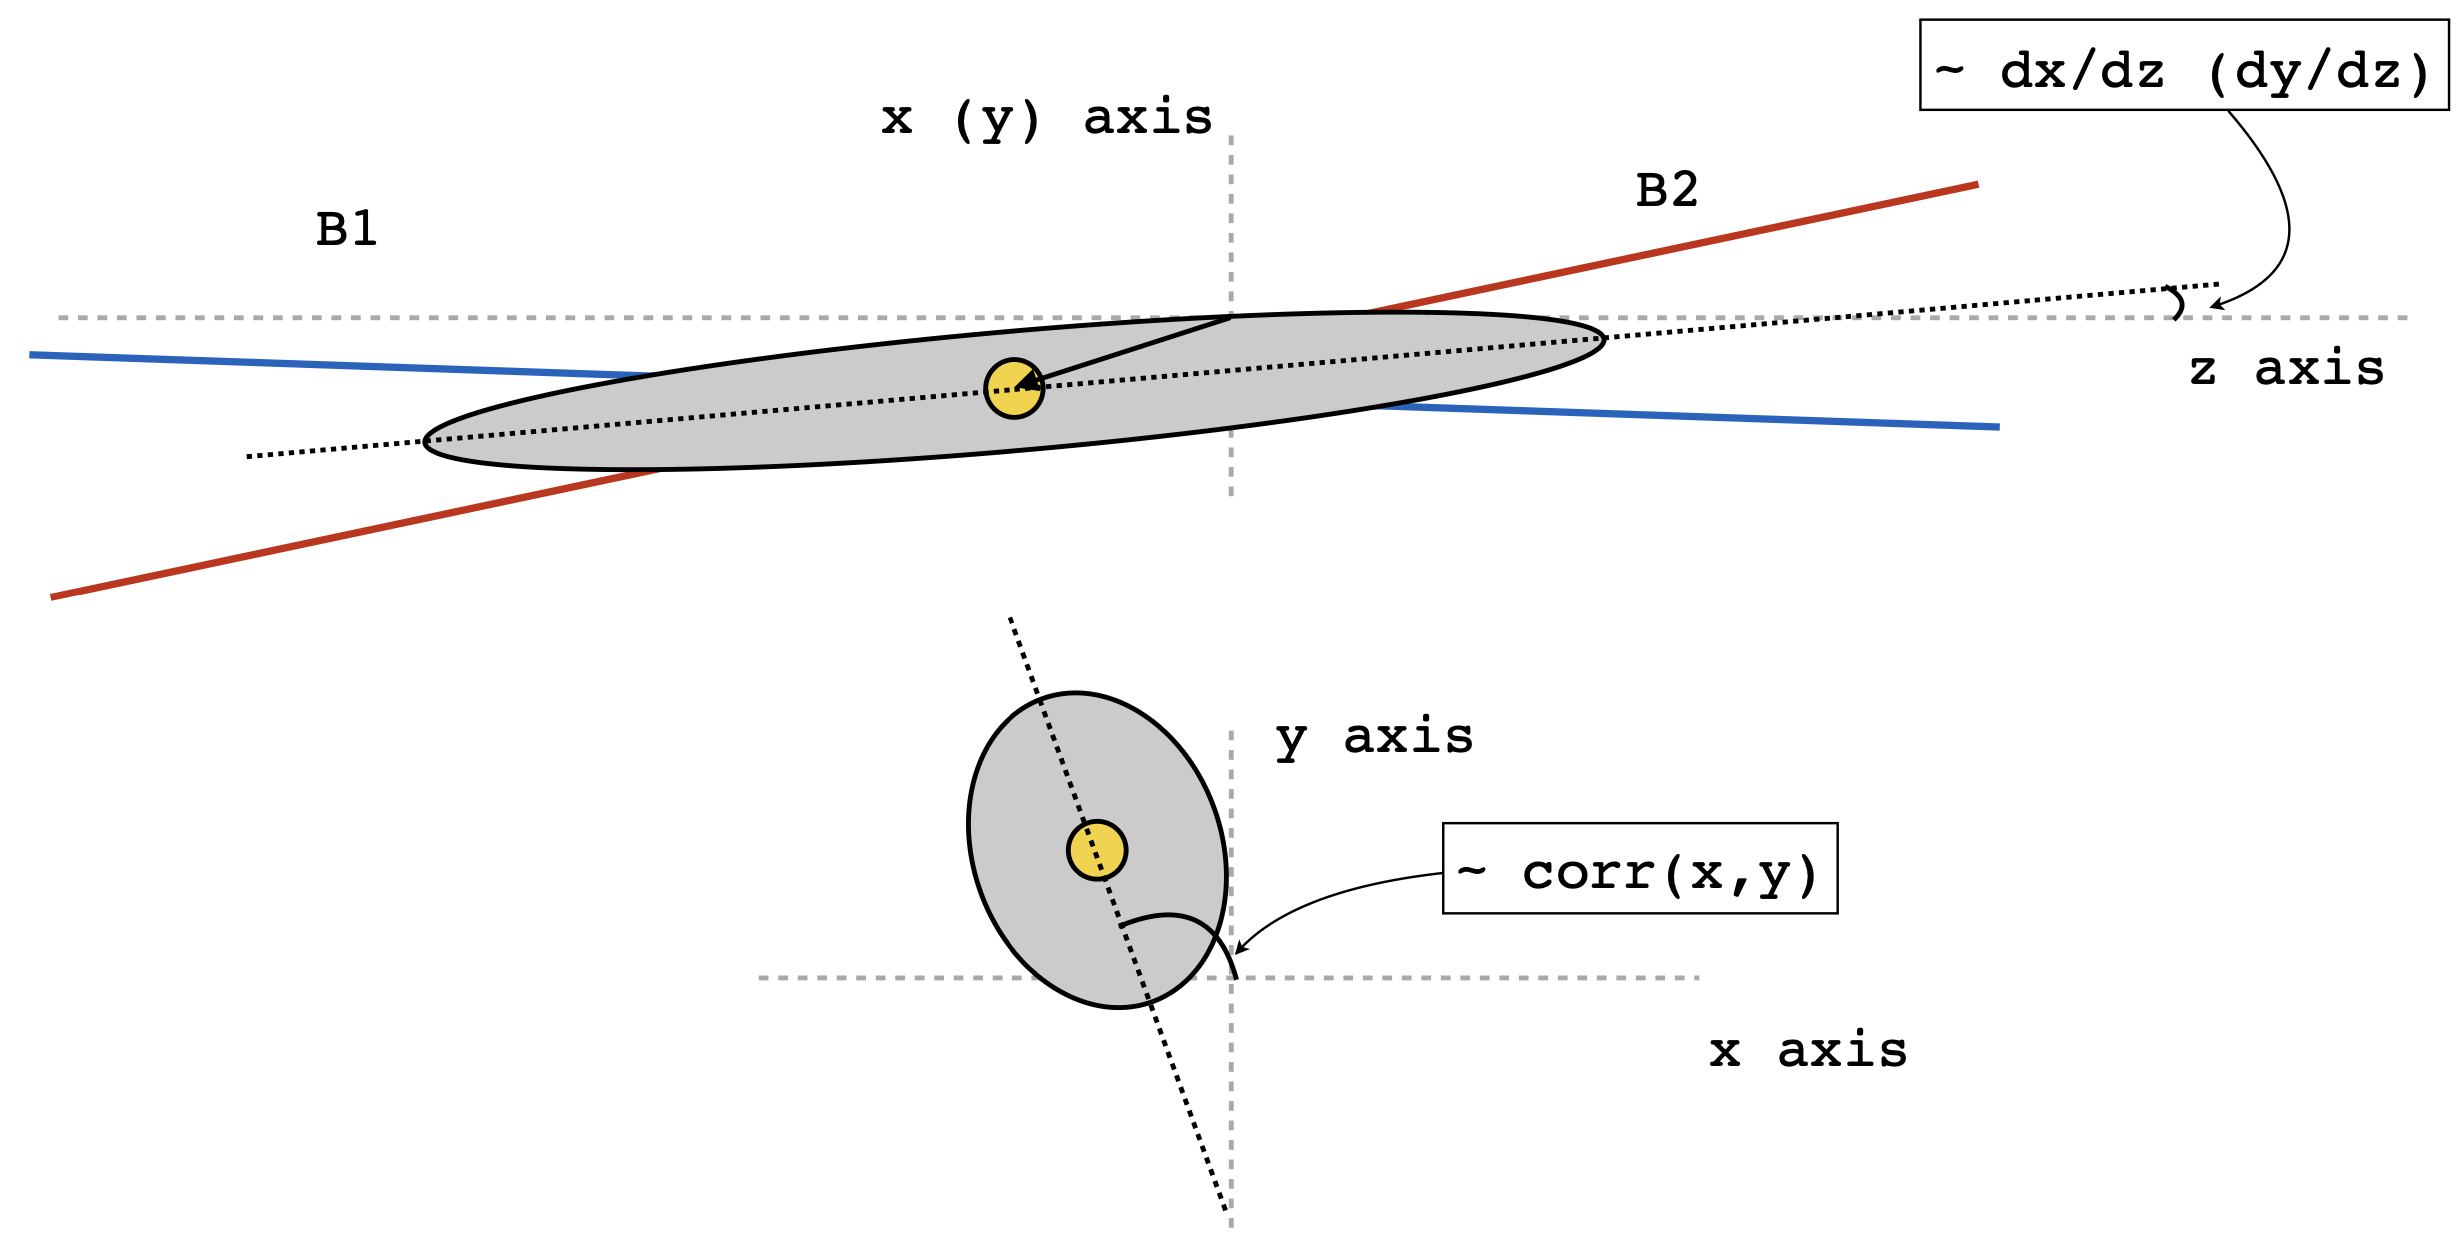
\includegraphics[width=0.7\textwidth]{figures/RealBeamspot.png}
   \caption{Diagram of the ideal (top) and real (bottom) beamspot.}
   \label{fig:beamspotCartoon}
\end{figure}

We determine the beamspot parameters by fitting track and vertex quantities for every lumi section.
The centroid position in the transverse plane and the tilts are obtained from a fit to the reconstructed tracks;
this is a $\chi^2$ fit that employs the track $d_0$--$\phi$ correlation:
\[
d_0(\phi_0, z_p) = x_{\text{BS}} \cdot \sin \phi_0 + \frac{dx}{dz} \cdot \sin\phi_0 \cdot z_p - y_{\text{BS}} \cdot \cos \phi_0 - \frac{dy}{dz} \cdot \cos \phi_0 \cdot z_p.
\]
as seen in Fig.~\ref{fig:trackD0Correlation}.

\begin{figure}[htbp]
   \centering
   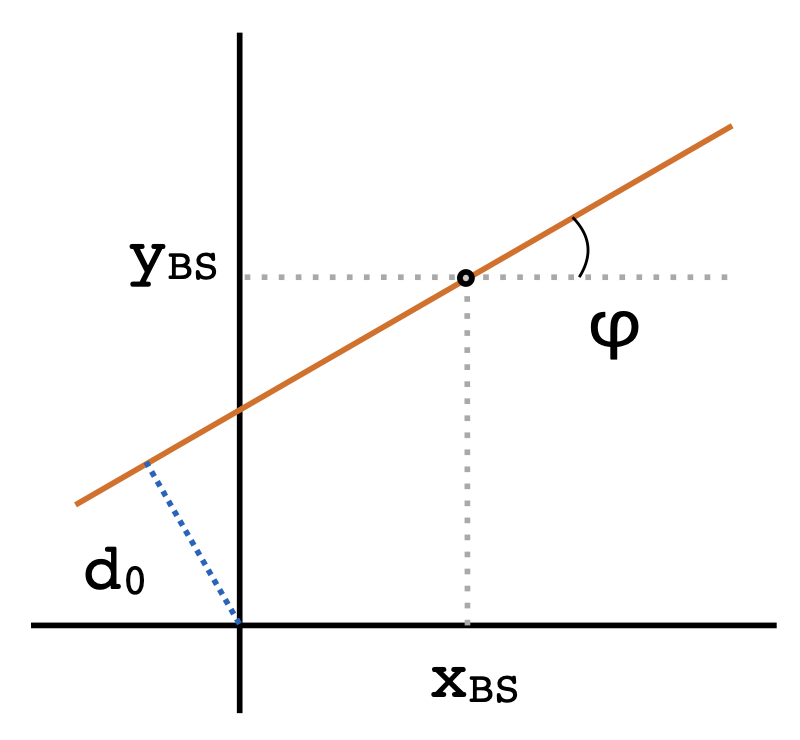
\includegraphics[width=0.5\textwidth]{figures/trackD0PhiCorrelation.png}
   \caption{The track $d_0$--$\phi$ can be used to measure the centroid position in the transverse plane and the centroid tilts.}
   \label{fig:trackD0Correlation}
\end{figure}

On the other hand,
the position along the $z$ axis and the beam widths are measured from a fit to the reconstructed vertices;
this is a maximum likelihood fit of a three-dimensional gaussian to the reconstructed vertices:
\[
\mathcal{L}=\sum_{\text {vertices }}-\ln \left(\frac{1}{\sqrt{(2 \pi)^3\left|\Sigma_{\text {tot }}\right|}} \cdot e^{-\frac{1}{2}(x-\mu)^T \Sigma_{\text {tot }}^{-1}(x-\mu)}\right)
\]
where $\Sigma_{\text {tot }} = \Sigma_{\text {beam }}^{\text {CMS }} + \Sigma_{\text {vtx }}$, with
$\Sigma_{\text {beam }}^{\text {CMS }}$ the beamspot widths in CMS's frame and
$\Sigma_{\text {vtx }}$ the vertex covariance matrix, different for every vertex.
Notice that $\Sigma_{\text {beam }}^{\text {CMS }}$ is rotated with respect to the beamspot principal axes:
\[
\Sigma_{\text {beam }}^{\text {CMS }}=R^T(\alpha, \beta, \gamma) \cdot \Sigma_{\text {beam }} \cdot R(\alpha, \beta, \gamma)
\]
where the $\alpha$ ($\beta$) rotation is along the $x$ ($y$) axis, and can be measured from $\frac{dy}{dz}$ ($\frac{dx}{dz}$).
The $\gamma$ rotation is negligible because the $xy$ correlation of the beams is very small.
The beamspot widths $\sigma_x$, $\sigma_y$, $\sigma_z$ are then given by the square roots of the diagonal elements of $\Sigma_{\text {beam }}$.

\subsubsection{Beamspot Workflows}

There are separated workflows for
online usage (in the HLT) and
offline usage (in the prompt reconstruction).
In the online case, there are again two separated workflows, both running in the DQM farm:
the \emph{HLT client} fit uses the the full tracks and vertices reconstructed in the HLT, whilst
the \emph{legacy client} fit uses pixel-only tracks and vertices fitted in the DQM clients themselves.
In both cases the payload is obtained through moving average over a five lumisections sliding window.
These payloads are uploaded to CondDB in a DQM "O2O-like" workflow,
and
are consumed both by the HLT processing and by the Express reconstruction.
In the HLT the conditions are fetched every five lumisections.
This workflow has an arbitration mechanism (via an \texttt{ESProducer}) between old and new payloads for dynamic selection, and the system is triggered whenever a tag is updated, ensuring robust operations.
The system also contains fallback mechanisms for edge cases:
\begin{itemize}
\item unavailability of tracks from the HLT,
\item failure of the beam fit,
\item long times since the last payload upload (default threshold: 1 day),
\item LHC machine transitions (\textit{e.g}., LS, TS, MD, pp $\leftrightarrow$ HI),
\item possibility of ``dummy'' beamspot / beamspot with inflated uncertainties if necessary.
\end{itemize}
In the offline case there are four PCL workflows.
The \emph{high purity} workflow runs off a set of well-measured vertices from a stream of high \HT events,
with stringent requirements on vertex \PT and number of tracks, whilst
the \emph{legacy} workflow runs on the regular Express stream and has minimal requirements on its inputs.
Both workflows have tags with lumisections and run granularity;
the standard tag used for prompt reconstruction is the high-purity by-lumisection tag, \texttt{BeamSpotObjects\_PCL\_byLumi\_v0\_prompt}.

\subsubsection{NGT Demonstrator Candidate Evaluation}
In view of the above discussion, the beamspot would be a natural candidate for the NGT calbirations.
Ideally we would like to bring the high-purity by-lumisection workflow to the online system,
but it is known that the pressure on the conditions delivery system may be problematic (hence the five-lumisection granularity).

%The Beamspot online workflow has been updated in Run 3 to address the absence of the SCAL system.\\
%This does not affect the actual fit to tracks or primary vertex distributions but modifies the infrastructure for handling BeamSpot information. Key changes include:
%\begin{itemize}
%    \item Replacement of SCAL-based processes.
%    \item Improved workflow and fallback mechanisms for edge cases.
%    \item Arbitration between old and new payloads for dynamic selection.
%\end{itemize}

%The old Run 2 workflow consisted in the following steps:
%\begin{itemize}
%    \item BeamSpot clients dumped data to text files processed through the SCAL system.
%    \item Data was forwarded to the DIP and HLT systems.
%\end{itemize}

%While the new workflow consists of the these steps:
%\begin{itemize}
%    \item SCAL system replaced by direct DB uploads.
%    \item An \texttt{ESProducer} arbitrates between BeamSpot payloads dynamically.
%    \item A fallback mechanism uses dummy values if no good payloads are available.
%    \item The system is triggered whenever a tag is updated, ensuring robust operations.
%\end{itemize}

%Failures in past workflows (e.g., due to unavailable tracks at HLT) necessitated a fallback mechanism. The %key features include:
%\begin{itemize}
%    \item Arbitration logic to decide between stored and new BeamSpot values.
%    \item Checks for fit convergence and recency of results.
%    \item Use of a 5-lumi-section sliding window for BeamSpot fits.
%    \item Ongoing studies on transverse widths, $\sigma_Z$, track counts, and PVs.
%\end{itemize}


%The new O2O mechanism ensures timely updates:
%\begin{itemize}
%    \item Automatically checks the time since the last payload upload (default threshold: 1 day).
%    \item Handles machine transitions (e.g., LS, TS, MD, pp $\leftrightarrow$ HI).
%    \item Uploads a "fake" BeamSpot object with inflated uncertainties if necessary.
%    \item Arbitration based on the time-of-creation of payloads, stored in \texttt{BeamSpotOnlineObjects}.
%\end{itemize}

%The updated Beam Spot online workflow addresses Run 3 requirements:
%\begin{itemize}
%    \item SCAL system replaced with DB uploads and fallback logic.
%    \item Successful implementation of O2O mechanisms for special machine transitions.
%    \item Ongoing work includes monitoring, fallback logic finalization, and integration with DIP.
%\end{itemize}
